\documentclass[../main.tex]{subfiles}





\begin{document}











































\chapter{Propietats de connexió}

En aquest capítol explorem la noció intuïtiva que un espai topològic sigui ``d'una peça''. Hi ha dues maneres de visualitzar aquesta idea: l'espai no es trenca en reunió de trossos oberts disjunts, o bé podem ``connectar per un camí'' qualsevol parella de punts de l'espai. Aquests dos punts de vista porten a les definicions d'espai connex i d'espai arc-connex, que, com veurem, no són equivalents. Comencem amb el concepte d'arc-connexió, ja que és un concepte més intuïtiu. La seva definició utilitza la topologia euclidiana sobre la recta real, contrastant-la amb la de l'espai topològic que s'estudia.


\section{Espais arc-connexos}
\subsection{Camins i espais arc-connexos}

\begin{defi}
[Camí]\index{Camí}\label{def:cami} Sigui $(X,\tau)$ un espai topològic. Un \textit{camí} en $X$ és una aplicació contínua $\alpha:I\rightarrow X$, on $I=[0,1]$. Diem que $\alpha(0)$ és el \textit{punt inicial} del camí i $\alpha(1)$ n'és el punt final. Si $\alpha(0) = \alpha(1)$ diem que el camí és tancat.
\end{defi}

\begin{defi}
[Arc-connex]\index{Arc-connex}\index{Espai arc-connex}\label{def:arcconnex} Un espai topològic $(X,\tau)$ és \textit{arc-connex} si per a tot $x,y\in X$ existeix un camí amb punt inicial $x$ i punt final $y$.
\end{defi}

\begin{ej}
\label{ej:arcconnex1} Considerem $X = (0,1)$ amb la topologia usual. Per a tot $x,y\in (0,1)$ definim una funció
\begin{equation}
    \notag
    \alpha:[0,1]\rightarrow (0,1),\qquad \alpha(t) = (1-t)x+ty
\end{equation}
Aleshores $\alpha$ és clarament contínua i $\alpha(0) = x$ i $\alpha(1) = y$. Per tant, és un camí i aleshores $\forall x,y\in X$ existeix un camí tal que $\alpha(0)=x$ i $\alpha(1) = y$. Per tant $X$ és arc-connex.
\end{ej}

\begin{ej}
\label{ej:arcconnex2} $\mathbb{R}^n$ és arc-connex. Si considerem $\forall x,y\in\mathbb{R}^n$, la mateixa aplicació d'abans
\begin{equation}
    \notag
    \begin{array}{rl}
        \alpha:I & \longrightarrow\mathbb{R}^n \\
        t & \longmapsto x+t(y-x)
    \end{array}
\end{equation}
veiem que és contínua i $\alpha(0) = x$ i $\alpha(1) = y$.
\end{ej}

\begin{ej}
\label{ej:arcconnex3} Pel teorema de Bolzano, tot camí $\alpha:I\rightarrow\mathbb{R}$ amb $\alpha(0)<0$ i $\alpha(1)>0$ passa pel 0. Per tant, $\mathbb{R}\setminus\{0\}$.
\end{ej}

\begin{ej}
\label{ej:arcconnex4} L'esfera $S^n$ és arc-connexa. En efecte, si $x,y\in S^n$, triem un punt $p\not=x$ i $p\not=y$. Per projecció estereogràfica $S^n\setminus\{p\}$ és homeomorf a $\mathbb{R}^n$, per tant, és arc-connex i existeix un camí a $S^n\setminus\{p\}$ (i per tant a $S^n$) amb inici a $x$ i final a $y$.
\end{ej}

\subsection{Propietats dels espais arc-connexos}

\begin{prop}
\label{prop:arcconnex1} Sigui $f:X\rightarrow Y$ una aplicació contínua i exhaustiva entre espais topològics. Si $X$ és arc-connex, $Y$ també ho és. En particular, un espai homeomorf a un espai arc-connex és arc-connex.
\end{prop}
\begin{proof}
Siguin $y_1,y_2\in Y$ i siguin $x_1,x_2\in X$ tals que $f(x_1) = y_1$ i $f(x_2) = y_2$. Com $X$ és arc-connex, existeix un camí $\alpha$ d'inici $x_1$ i final $x_2$. Aleshores $f\circ \alpha$ és un camí d'inici $y_1$ i final $y_2$.
\end{proof}

\begin{coro}
\label{coro:rirnnosonhomeomorfs} $\mathbb{R}$ i $\mathbb{R}^n$ no són homeomorfs.
\end{coro}
\begin{proof}
Si existís un homeomorfisme $f:\mathbb{R}\longrightarrow \mathbb{R}^n$, aleshores $\mathbb{R}\setminus\{0\}$ seria homeomorf a $\mathbb{R}^n\setminus\{f(0)\}$ però el primer espai no és arc-connex per (\ref{ej:arcconnex3}) i el segon sí.
\end{proof}

\begin{prop}
\label{prop:arcconnex2} Siguin $X,Y$ espais topològics. El producte $X\times Y$ és arc-connex si i només si $X$ i $Y$ són arc-connexos.
\end{prop}
\begin{proof}
Si $X\times Y$ és arc-connex, aplicant la proposició anterior (\ref{prop:arcconnex1}) a les aplicacions
\begin{equation}
    \notag
    \pi_X:X\times Y\longrightarrow X\qquad \pi_Y:X\times Y\longrightarrow Y
\end{equation}
(que són funcions contínues i exhaustives) obtenim que $X$ i $Y$ són arc-connexes.

Recíprocament, suposem que $X$ i $Y$ són arc-connexos i siguin $(x_1,y_1),(x_2,y_2)\in X\times Y$. Siguin $\sigma,\eta$ camins a $X$ i $Y$ respectivament, tals que $\sigma(0) = x_1$, $\sigma(1) = x_2$ i $\eta(0) = y_1$ i $\eta(1) = y_2$. Aleshores
\begin{equation}
    \notag
    \begin{array}{rl}
        f:I & \longrightarrow X\times Y \\
        t & \longmapsto (\sigma(t),\eta(t))
    \end{array}
\end{equation}
és un camí amb punt inicial $(x_1,y_1)$ i punt final $(x_2,y_2)$.
\end{proof}

\begin{defi}
\label{def:productedecamins} Definim el producte de dos camins $\sigma\cdotp\eta$ de la següent manera:
\begin{equation}
    \notag
    \sigma\cdotp\eta:I\longrightarrow X,\quad (\sigma\cdotp\eta)(t) = \left\{
    \begin{array}{lll}
        \sigma(2t) & \text{si} & 0\leq t\leq 1/2 \\
        \eta(2t-1) & \text{si} & 1/2\leq t\leq 1
    \end{array}
    \right.
\end{equation}
\end{defi}

\begin{prop}
\label{prop:arcconnex3} Sigui $X$ un espai topològic i sigui $\{A_i\}_{i=1}^\infty$ una col·lecció numerable (no té per què ser finita) de subespais arc-connexos de $X$. Si $A_i\cap A_{i+1}\not=\emptyset$, $\forall i=1,\ldots$, aleshores $\bigcup_{i=1}^\infty A_i$ és arc-connex.
\end{prop}
\begin{proof}
Sigui $\{A-i\}_{i=1}^\infty$ una família numerable de subespais arc-connexos de $X$. $\forall i\in\{1,2,\ldots\}$ sigui $a_i\in A_i\cap A_{i+1}$ que és possible ja que per hipòtesis $A_i\cap A_{i+1}\not=\emptyset$. Ara, com que $A_i$ és connex, existeix un camí $\alpha_i:I\rightarrow X$ tal que $\alpha_i(0) = a_i$, $\alpha_i(1) = a_{i+1}$. Siguin ara $x,y\in\bigcup_{i=1}^\infty A_i$, $x\not=y$. Aleshores, $\exists j,k\in\{1,2,\ldots\}$ tals que $x\in A_j$ i $y\in A_k$. Podem assumir, sense pèrdua de generalitat, que $j<k$. Aleshores, existeixen camins $\eta_1,\eta_2:I\rightarrow X$ tals que $\eta_1(0)=x$ i $\eta_1(1) = a_j$, mentre $\eta_2(0)=a_k$ i $\eta_2(1) = y$. Considerem el següent camí:
\begin{equation}
    \notag
    \eta_1\cdotp\alpha_j\cdotp\alpha_{j+1}\cdotp\cdots\cdotp\alpha_{k-1}\cdotp\alpha_k\cdotp\eta_2
\end{equation}
\begin{equation}
    \notag
    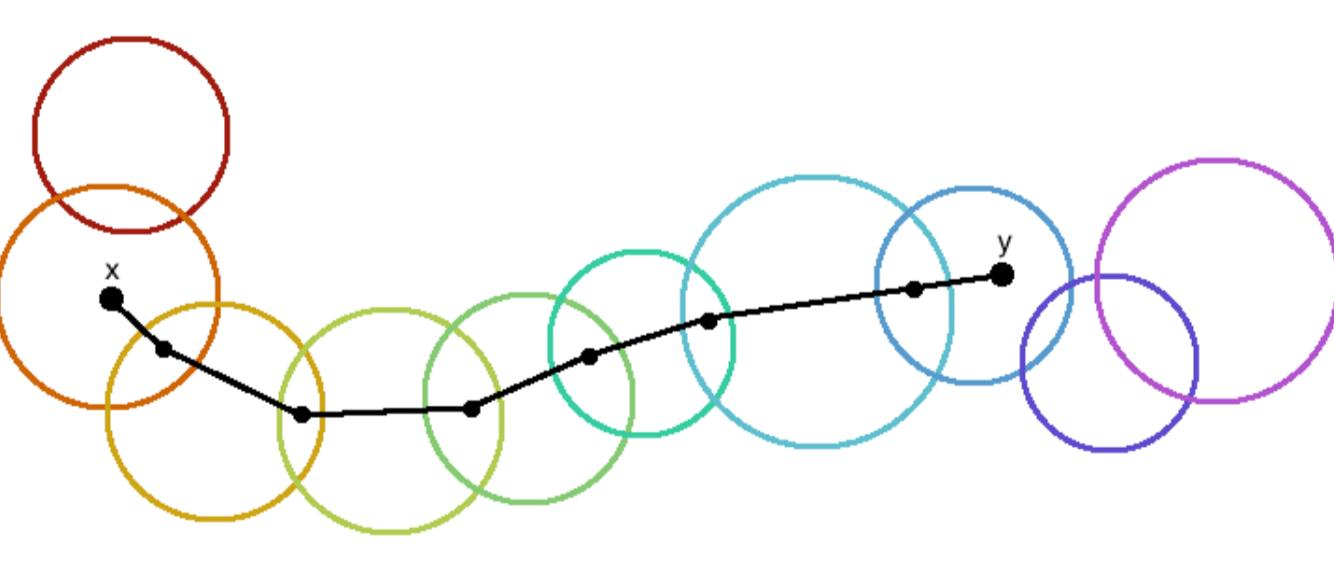
\includegraphics[scale = 0.3]{fotos_topo_1/unioarcconnexos.jpeg}
\end{equation}
Aleshores és un camí de $x$ a $y$, per tant $\bigcup_{i=1}^n A_i$ és arc-connex.
\end{proof}

\subsection{Components arc-connexes}

\begin{defi}
[Arc-connectats]\index{Arc-connectats}\label{def:arcconnectats} Sigui $(X,\tau)$ un espai topològic. Diem que dos punts $x,y\in X$ estan \textit{arc-connectats} si existeix un camí amb punt inicial $x$ i punt final $y$.
\end{defi}

\begin{prop}
\label{prop:larelaciodarcconnexioesdequivalencia} La relació $x$ ``arc-connectat amb'' $y$ és d'equivalència.
\end{prop}
\begin{proof}
Veiem que compleix les tres propietats: reflexivitat, simetria i transitivitat.
\begin{enumerate}[(i)]
    \item És reflexiva, atès que les aplicacions constants són contínues.
    \item Si $\sigma:I\rightarrow X$ és tal que $\sigma(0) = x$ i $\sigma(1) = y$, aleshores la composició:
    \begin{equation}
        \notag
        \begin{array}{rl}
            \overline{\sigma}:I\rightarrow I & \overset{\sigma}{\longrightarrow} X \\
            t & \longmapsto 1-t
        \end{array}
    \end{equation}
    és contínua, $\overline{\sigma}(0)=y$ i $\overline{\sigma}(1) = x$; per tant es verifica la propietat simètrica.
    \item Veiem finalment que és transitiva:
    \begin{itemize}
        \item $x$ arc-connectat amb $y$ $\Rightarrow \exists$ camí $\sigma:I\rightarrow X$ tal que $\sigma(0) = x$ i $\sigma(1) = y$.
        \item $y$ arc-connectat amb $z$ $\Rightarrow \exists$ camí $\eta:I\rightarrow X$ tal que $\eta(0) = y$ i $\eta(1) = z$.
    \end{itemize}
    
    Aleshores prenem la definició (\ref{def:productedecamins}) i com que $\sigma(2\cdotp\frac{1}{2}) = \sigma(1) = y = \eta(0) = \eta(2\cdotp\frac{1}{2}-1)$, l'aplicació $\sigma\cdotp\eta$ és contínua i
    \begin{equation}
        \notag
        (\sigma\cdotp\eta)(0) = \sigma(0) = x,\qquad (\sigma\cdotp\eta)(1) = \eta(1)=z
    \end{equation}
    Per tant $x$ està arc-connectat amb $z$ pel camí $\sigma\cdotp\eta$.
\end{enumerate}
\end{proof}

\begin{defi}
[Component arc-connexa]\index{Component arc-connexa} Sigui $X$ un espai topològic i sigui $x\in X$. La component arc-connexa de $x$ és
\begin{equation}
    \notag
    ca(x):=\{y\in X\;:\;\text{$x$ està arc-connectat amb $y$}\}
\end{equation}
\end{defi}

Així, $X$ és reunió disjunta de components arc-connexes. Òbviament $X$ és arc-connex si i només si té una única component arc-connexa.

\begin{ej}
\label{ej:componentsarcconnexes} Exemples
\begin{enumerate}
    \item $\mathbb{R}^2\setminus\{(x,y)\;:\;y=0\}$ té dues components arc-connexes.
    \item Considerem $\mathbb{Q}$ amb la topologia induïda per $\mathbb{R}$. Aleshores, per a tot $q\in\mathbb{Q}$, $ca(q) = \{q\}$.
\end{enumerate}
\end{ej}

\begin{prop}
\label{prop:subespaiarcconnexmesgranquecontex} Sigui $X$ un espai topològic i sigui $x\in X$. La component arc-connexa $ca(x)$ és el subespai arc-connex més gran que conté $x$.
\end{prop}
\begin{proof}
Veiem primer que $ca(x)$ és arc-connex; si $y\in ca(x)$, aleshores existeix un camí $\sigma:I\rightarrow X  $ tal que $\sigma(0) = x$ i $\sigma(1) = y$. Cal veure que $\sigma(I)\subset ca(x)$. En efecte, si $y=\sigma(t)$, aleshores
\begin{equation}
    \notag
    \begin{array}{rl}
        \overline{\sigma}:I & \rightarrow X \\
        s & \longmapsto \sigma(s\cdotp t)
    \end{array}
\end{equation}
és contínua i $\overline{\sigma}(0)=\sigma(0)=x$, $\overline{\sigma}(1)=\sigma(t)=y$. Per tant $y\in ca(x)$. 

Sigui ara $A\subset X$ un subespai arc-connex tal que $x\in A$. Per a tot punt $y\in A$, $y$ està arc-connectat amb $x$ a $A$ i, per tant, també a $X$. En conseqüència, $y\in ca(x)$.
\end{proof}

\subsection{Localment arc-connex}

\begin{defi}
[Localment arc-connex]\label{def:localmentarcconnex}\index{Localment arc-connex} Un espai topològic $X$ es diu \textit{localment arc-connex} si per a tot punt $x\in X$ i tot entorn $U$ de $x$ existeix un entorn arc-connex de $x$ contingut en $U$.
\end{defi}

Alternativament, i recuperant la definició de \textit{localment P}, on $P$ simbolitza una propietat sobre un espai topològic, podríem dir que un espai topològic $X$ és localment arc-connex, si per a tot punt $x\in X$ existeix una base d'entorns arc-connexos.

\begin{ej}
\label{ej:localmentarcconnex} $\mathbb{R}^n$ és arc-connex (per tant és localment arc-connex). $X = \{(0,y)\;:\;y\in[-1,1]\}\cup\{(x,\sin(\pi/x))\;:\;x\in(0,1]\}$ no és localment arc-connex en els punts de la forma $(0,x),\;-1\leq x\leq 1$.
\begin{equation}
    \notag
    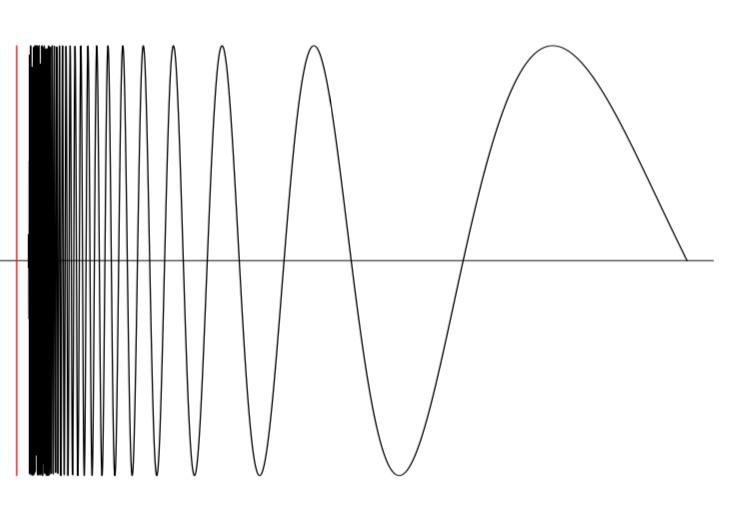
\includegraphics[scale = 0.3]{fotos_topo_1/localmentarcconnex.jpeg}
\end{equation}
\end{ej}


\section{Espais connexos}
\subsection{Definició i exemples}

\begin{defi}
[Connex]\label{def:connex}\index{Connex}\index{Espai connex} Sigui $X$ un espai topològic. Diem que $X$ és \textit{connex} si no es pot expressar com a unió de dos oberts disjunts no buits. És a dir, $X$ és connex si $X = U\cup V$, amb $U,V$ oberts tals que $U\cap V = \emptyset$, implica que $U=\emptyset$ o bé $V = \emptyset$.
\end{defi}

\begin{equation}
    \notag
    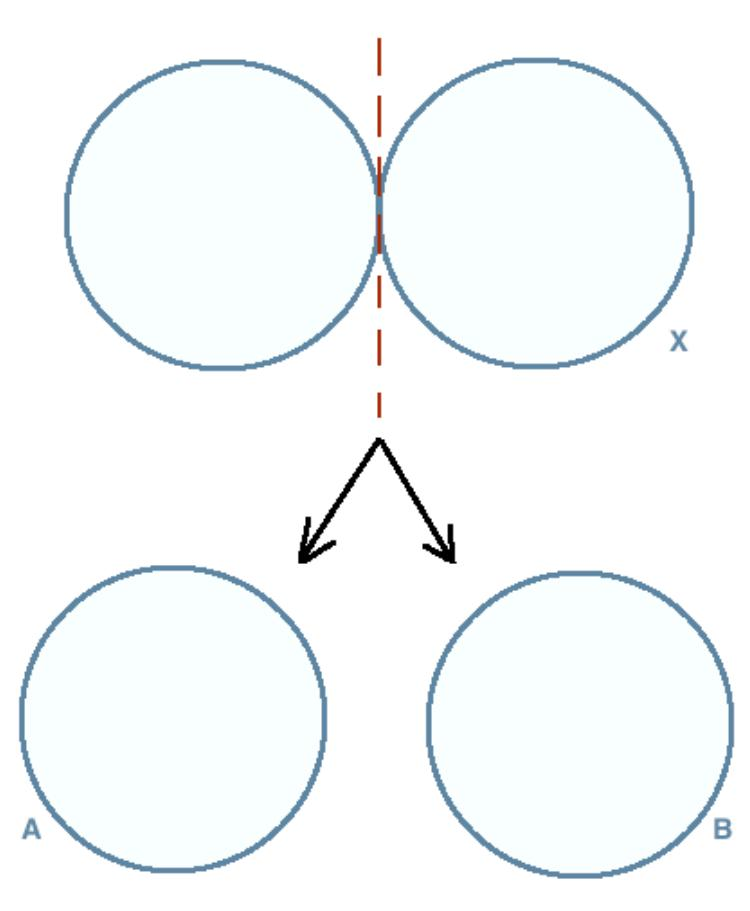
\includegraphics[scale = 0.3]{fotos_topo_1/espaiconnex.jpeg}
\end{equation}

De vegades es diu que $\{U,V\}$ és una separació de $X$, si $U,V\not=\emptyset$ són oberts tals que $U\cap V = \emptyset$ i $X = U\cup V$.

\begin{ej}
\label{ej:connex1} Considerem l'espai topològic $\mathbb{R}$ amb la topologia euclidiana. Considerem el subespai topològic $\mathbb{Q}$. Afirmem que $\mathbb{Q}$ és un espai topològic no connex.

En efecte, considerem $\sqrt{2}\in\mathbb{R}$ i considerem els subconjunts
\begin{equation}
    \notag
    A = \{q\in\mathbb{Q}\;:\;q<\sqrt{2}\},\qquad B = \{q\in\mathbb{Q}\;:\;q>\sqrt{2}\}
\end{equation}
Afirmem que $\{A,B\}$ és una separació de $\mathbb{Q}$. Primer notem que $A$ i $B$ són oberts de $\mathbb{Q}$, ja que $A = \mathbb{Q}\cap (-\infty,\sqrt{2})$ i $B = \mathbb{Q}\cap(\sqrt{2},+\infty)$, amb $(-\infty,\sqrt{2}),(\sqrt{2},\infty)\subset\mathbb{R}$ oberts de $\mathbb{R}$. (Recordem de la topologia subespai com eren els oberts (\ref{def:topologiasubespai2.0}), (\ref{def:subespaitopologic})). A més, $A$ i $B$ són no buits ja que, per exemple, $0\in A$ i $2\in B$. Finalment veiem que $A\cap B=\emptyset$ ja que $\nexists q\in\mathbb{Q}$ tal que $q<\sqrt{2}$ i $q>\sqrt{2}$ a la vegada. Per últim, no és difícil veure que $\mathbb{Q} = A\cup B$.
\end{ej}

Demostrar que un espai topològic és connex és molt més difícil que demostrar que no ho és. Per això, al final veure que arc-connex implica connex i és molt més fàcil veure que és arc-connex.

\begin{ej}
\label{ej:connex2} $\mathbb{R}$ és connex. En efecte, si $\mathbb{R} = U\cap V$ amb $U$ i $V$ oberts no buits disjunts, aleshores l'aplicació
\begin{equation}
    \notag
    \begin{array}{rll}
        f:\mathbb{R} & \longrightarrow\mathbb{R} & \\
        x & \longmapsto 1 & \text{si}\;x\in U \\
        x & \longmapsto -1 & \textit{si}\;x\in V
    \end{array}
\end{equation}
és contínua, la qual cosa contradiu el Teorema de Bolzano. Amb el mateix argument obtenim que els intervals oberts i els tancats són connexos.
\end{ej}

\begin{ej}
\label{ej:connex3} $X = \mathbb{R}^2\setminus\{(x,y)\in\mathbb{R}^2\;:\;y=0\}$ no és connex. En efecte, podem escriure $X = X^+\cup X^-$, on $X^+ = \{(x,y)\in\mathbb{R}^2\;:\;y>0\}$ i $X^- = \{(x,y)\in\mathbb{R}^2\;:\;y<0\}$ són oberts no buits i $X*+\cap X^-=\emptyset$.
\end{ej}

\subsection{Criteris de connexió}

\begin{prop}
\label{prop:criterideconnexio1} Un espai topològic $X$ és connex si i només si els únics subconjunts oberts i tancats\footnote{En anglès, aquests conjunts es diuen ``clopen'', \textit{close and open}.} de $X$ són $X$ i $\emptyset$.
\end{prop}
\begin{proof}
Suposem que $X$ és connex i sigui $A\subseteq X$ obert i tancat. Com $A$ és obert, $X\setminus A$ és tancat, i com $A$ és tancat, $X\setminus A$ és obert. Aleshores $X = A\cup(X\setminus A)$ és una unió disjunta de dos oberts. Com $X$ és connex, ha de ser $A = \emptyset$ o bé $X\setminus A = \emptyset\Rightarrow A = X$.

Recíprocament, suposem $X = U\cup V$ on $U$ i $V$ són oberts disjunts, aleshores $U$ és obert i tancat, ja que $X\setminus U = V$ que és obert, i per tant $U=\emptyset$ o bé $U = X$, que implica que $X$ és connex.  
\end{proof}

\begin{prop}
\label{prop:criterideconnexio2} Sigui $X$ un espai topològic i sigui $\{0,1\}$ l'espai topològic amb la topologia discreta. Aleshores $X$  no és connex si i només si existeix una funció contínua i exhaustiva $f:X\rightarrow \{0,1\}$
\end{prop}
\begin{equation}
    \notag
    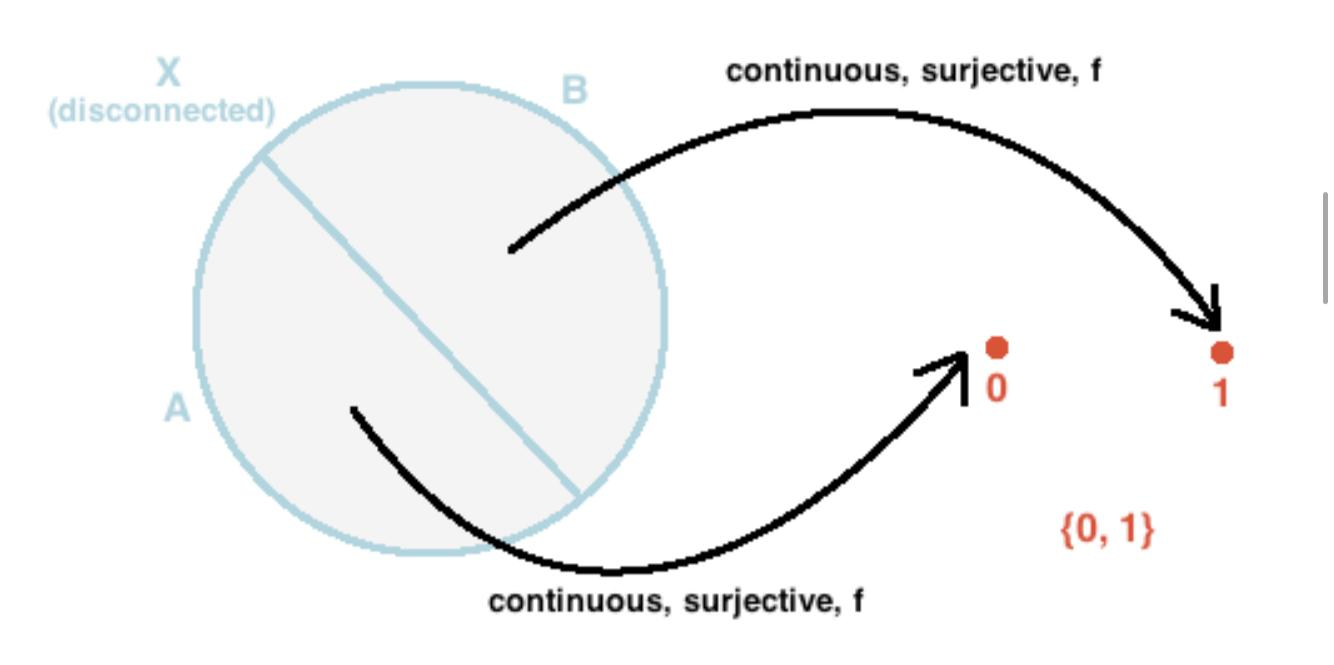
\includegraphics[scale = 0.3]{fotos_topo_1/f01.jpeg}
\end{equation}
\begin{proof}
\begin{itemize}
    \item ($\Rightarrow$) Suposem que $X$ és un espai topològic no connex. Aleshores existeixen $A,B\subset X$ oberts no buits tals que $A\cap B = \emptyset$ i $A\cup B =X$. Definim la funció següent:
    \begin{equation}
        \notag
        f:X\rightarrow \{0,1\},\quad f(x) = \left\{
        \begin{array}{lll}
            0 & \text{si} & x\in A\\
            1 & \text{si} & x\in B
        \end{array}
        \right.
    \end{equation}
    Clarament $f(X) = \{0,1\}$ i per tant és exhaustiva. Veiem que sigui contínua. Com $\{0,1\}$ té la topologia discreta, tot subconjunt de $\{0,1\}$ és un obert. Més precisament, $\emptyset,\{0\},\{1\}$ i $\{0,1\}$ són oberts de $\{0,1\}$. Notem que
    \begin{equation}
        \notag
        f^{-1}(\emptyset) = \emptyset,\quad f^{-1}(\{0\}) = A,\quad f^{-1}(\{1\}) = B,\quad f^{-1}(\{0,1\}) = A\cup B = X
    \end{equation}
    En tots els casos és un obert de $X$, ergo $f$ és contínua.
    
    \item ($\Leftarrow$) Suposem que existeix una aplicació contínua i exhaustiva $f:X\rightarrow \{0,1\}$. Afirmo que $\{f^{-1}(\{0\}),f^{-1}(\{1\})\}$ és una separació de $X$. En efecte, com que $f$ és contínua i $\{0,1\}$ està amb la topologia discreta, $f^{-1}(\{0\})$ i $f^{-1}(\{1\})$ són oberts en $X$, que a més són no buits per l'exhaustivitat de $f$. D'altra banda, 
    \begin{equation}
        \notag
        \emptyset = f^{-1}(\emptyset) = f^{-1}(\{0\}\cap\{1\}) = f^{-1}(\{0\})\cap f^{-1}(\{1\})
    \end{equation}
    i finalment, com $\{0,1\} = \{0\}\cup\{1\}$, aleshores $X = f^{-1}(\{0,1\}) = f^{-1}(\{0\}\cup\{1\}) = f^{-1}(\{0\})\cup f^{-1}(\{1\})$
\end{itemize}
\end{proof}

\subsection{Subespais connexos}

\begin{defi}
[Subespai connex]\label{def:subespaiconnex}\index{Subespai connex} Sigui $X$ un espai topològic i $A\subseteq X$ un subespai (amb la topologia subespai). Es diu que $A$ és un \textit{subespai connex} si és un espai topològic connex respecte la topologia subespai. De igual manera, es dirà que és inconnex o no connex si ho és com a espai topològic amb la topologia subespai.
\end{defi}

\begin{ej}
\label{ej:subespaiconnex} Considerem l'espai topològic $\mathbb{R}$ amb la topologia euclidiana. Sigui $A = (0,1)\cup [2,3]$. Aleshores, $A$ amb la topologia subespai és un espai topològic inconnex.
\begin{equation}
    \notag
    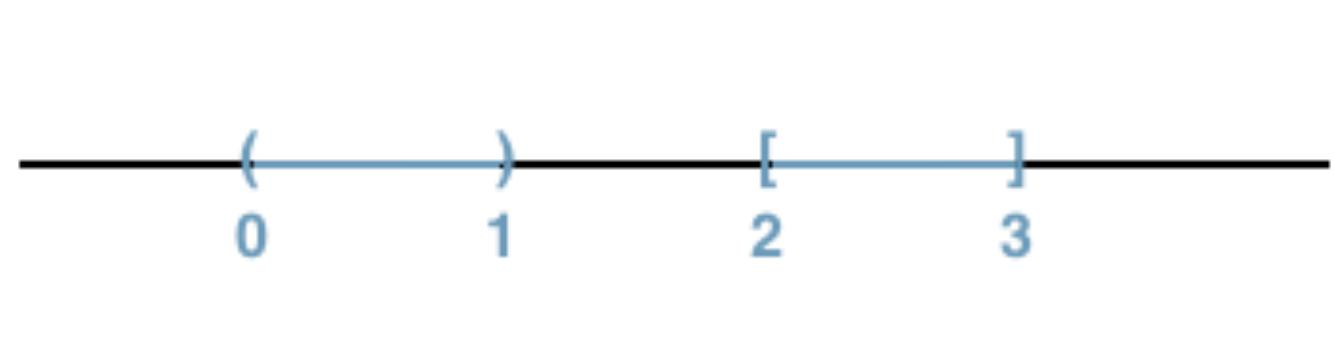
\includegraphics[scale = 0.3]{fotos_topo_1/exemplesubespaiconnex.jpeg}
\end{equation}

En efecte, sigui $B = (0,1)$ i $C= [2,3]$. Clarament $B,C\subset A$, $B\cap C = \emptyset$ i $B\cup C = A$, $B,C\not=\emptyset$. Només queda veure que $B$ i $C$ són oberts en $A$. Recordem que la topologia subespai té per oberts les interseccions d'$A$ amb els oberts de $\mathbb{R}$. Veiem, doncs, 
\begin{equation}
    \notag
    (0,1)\cap A = (0,1) = B,\qquad (3/2, 4)\cap A = [2,3] = C
\end{equation}
i per tant $B$ i $C$ són oberts en $A$ amb la topologia subespai. Això prova que $\{B,C\}$ és una separació d'$A$, ergo $A$ no és connex.
\end{ej}

\begin{prop}
\label{prop:clausuratambeconnexa} Sigui $X$ un espai topològic i $A\subseteq X$. Si $A$ és connex, aleshores $\overline{A}$ també ho és.
\end{prop}
\begin{proof}
Sigui $A$ un subespai topològic connex i suposem $\overline{A}$ inconnex. Aleshores existeixen oberts $B,C\subset \overline{A}$ tals que $B,C\not=\emptyset$, $B\cap C=\emptyset$ i $B\cup C=\overline{A}$. Com $\overline{A}=B\cup C$, prenem la clausura a ambdues bandes:
\begin{equation}
    \notag
    \overline{A} = \overline{\overline{A}} = \overline{B\cup C}=\overline{B}\cup \overline{C}.
\end{equation}
Això ens fa veure que $B = \overline{B}$ i $C = \overline{C}$. Així doncs, $B$ i $C$ són oberts i tancats de $A$. Ara, com $A\subseteq \overline{A}$, $A = (B\cap A)\cup (C\cap A)$. Aleshores $B\cap A$ i $C\cap A$ són oberts. Com $A$ és connex, algun dels dos ha de ser $\emptyset$. Suposem $A\cap B = \emptyset$. Aleshores $A = A\cap C\Rightarrow A\subseteq C\Rightarrow A \subseteq \overline{C}$. Prenent clausura a ambdues bandes $\overline{A}\subseteq \overline{C}$ però aleshores $\overline{A}=\overline{C}$ (ja que $\overline{C}\subseteq \overline{A}$) i això és una contradicció. De la mateixa manera, si suposem que $A\cap C = \emptyset$ arribem a la mateixa contradicció. Finalment, doncs, $\overline{A}$ no pot ser inconnex.
\end{proof}

\subsection{Criteris de connexió de subespais}

Sigui $X$ un espai topològic i siguin $\{A_i\}_{i\in I}$ una família arbitrària de subespais connexos, aleshores $\bigcup_{i\in I} A_i$ no té per què ser connex. Ara estudiarem quan és connex. Per exemple, considerem l'espai topològic $\mathbb{R}$ i sigui $A_n = (2n-1,2n)$, $\forall n\in\mathbb{N}$. Considerem la família
\begin{equation}
    \notag
    \{A_i\}_{i\in\mathbb{N}} = \{(1,2),(3,4),(5,6),\ldots\}
\end{equation}
Tots els $A_n$ són connexos clarament, però la reunió $\bigcup_{n=1}^\infty (2n-1,2n)$ és clarament inconnexa. Per demostrar-ho, podem prendre $A = (1,2)$ i $B = \bigcup_{n=2}^\infty (2n-1,2n)$ i clarament $\{A,B\}$ és una separació de $\bigcup_{n=1}^\infty A_n$.

\begin{prop}
\label{prop:subespaisconnexos1} Sigui $X$ un espai topològic i sigui $\{A_i\}_{i\in I}$ una família arbitrària de subespais connexos. Si $\bigcap_{i\in I}A_i\not=\emptyset$, aleshores $\bigcup_{i\in I}A_i$ és connex.
\end{prop}
\begin{equation}
    \notag
    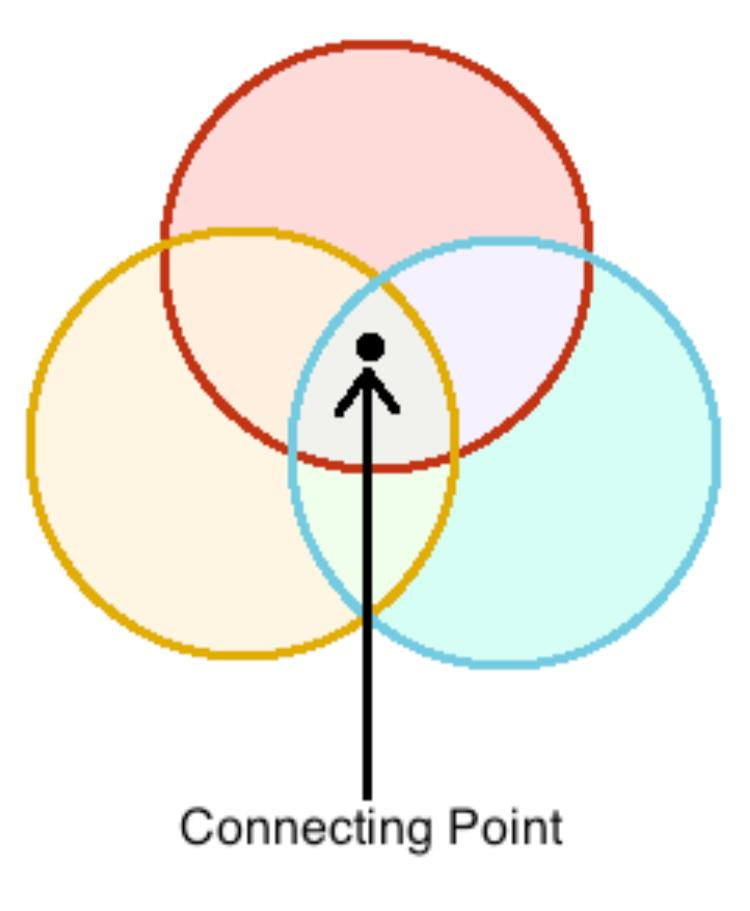
\includegraphics[scale = 0.3]{fotos_topo_1/puntconnector.jpeg}
\end{equation}
\begin{proof}
Suposem que $\bigcup_{i\in I} A_i$ és inconnex. Aleshores existeix un conjunt $B\subseteq \bigcup_{i\in I}A_i$ que és obert i tancat a l'hora tal que $B\not=\emptyset$ i $B\not=\bigcup_{i\in I}A_i$. Sigui $j\in I$. Suposem $B\cap A_j\not=\emptyset$. Veurem que $A_j\subseteq B$. Suposem que $A_j\not\subseteq B$. Com $B$ és un obert en $\bigcup_{i\in I}A_i$ això implica que $B\cap A_j$ és un obert no buit de $A_j$. Però com $B$ és també tancat, $B^c$ és un obert no buit de $A_j$. Però llavors
\begin{equation}
    \notag
    (B\cap A_j)\cap (B^c\cap A_j) = \emptyset\quad \text{i}\quad A_j = (B\cap A_j)\cup (B^c\cap A_j)
\end{equation}
i hem dit que $A_j$ era connex, per tant això no pot ser i per tant $A_j\subseteq B$.

Per tant, $\exists J\subseteq I$ tal que $B =  \bigcup_{i\in J}A_i$. Ara, com $B\not=\bigcup_{i\in I} A_i$, $\exists k\in I\setminus J$ tal que $A_k\not\subseteq B$. Tenim que $\cap_{i\in I}A_i\not=\emptyset$ i $B\cap A_k = \emptyset$. Aleshores, per la mateixa raó d'abans, $\{B\cap A_k,B^c\cap A_k\}$ és una separació d'$A_k$ però $A_k$ és connex, per tant no pot ser. Així doncs, $\bigcup_{i\in I}$ és connex.
\end{proof}

En aquesta proposició hem vist que si tenim una família arbitrària de subconjunts connexos, la unió d'aquests és un subconjunt connex si aquests tenen un punt en comú. Ara bé, aquesta no és l'única manera en què la unió sigui connexa. A continuació veurem que si tots els subespais intersequen amb un de comú, aleshores la unió serà connexa.

\begin{prop}
\label{prop:subespaisconnexos2} Sigui $X$ un espai topològic i sigui $\{A_i\}_{i\in I}$ una família arbitrària de subespais topològics connexos. Si $A_0$ és un altre subespai connex i $A_0\cap A_i\not=\emptyset$ $\forall i\in I$, aleshores $A_0\cup\bigcup_{i\in I}A_i$ és connex.
\end{prop}
\begin{equation}
    \notag
    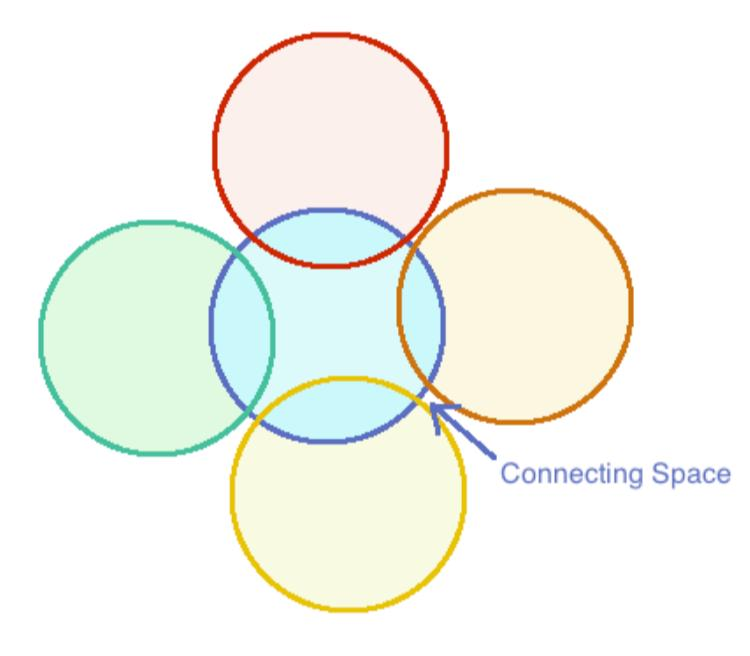
\includegraphics[scale = 0.3]{fotos_topo_1/espaiconnector.jpeg}
\end{equation}
\begin{proof}
Suposem que, donades les hipòtesis, $A = A_0\cup\bigcup_{i\in I}A_i$ és inconnex. Aleshores, existeix $B\subseteq A$ obert i tancat tal que $B\not=\emptyset,A$. Sigui $j\in I\cup\{0\}$ i suposem que $B\cap A_j\not=\emptyset$ (i/o $B\cap A_0\not=\emptyset$). A la demostració de la proposició anterior ja hem establert que $A_j\subseteq B$ (i/o $A_0\subseteq B$) ja que sinó podríem generar una separació de $A_j$ (i/o $A_0$) i contradiu que és connex. Veiem doncs, que $\exists J\subseteq I$ pel qual 
\begin{equation}
    \notag
    B = \bigcup_{i\in J}A_i
\end{equation}
Considerem dos casos:
\begin{enumerate}[1)]
    \item Si $A_0\subseteq B$. Aleshores $B\cap A_i\not=\emptyset$ $\forall i\in I$. Per tant, $B = A_0\cup\bigcup_{i\in I}A_i$. Això contradiu el fet que $B\not=A$.
    \item Si $A_0\not\subseteq B$. Això implica que $A_0\cap B = \emptyset$. Però $A_0\cap A_i\not=\emptyset$ $\forall i\in I$, i com $B$ és unió dels $A_i$'s això és una contradicció.
\end{enumerate}
En els dos casos arribem a una contradicció. Per tant, $A$ no pot ser inconnex.
\end{proof}

\begin{lema}
\label{lema:recobrimentsconnex} Sigui $X$ un espai topològic i sigui $\{X_i\}_{i\in I}$ un recobriment tal que $X_i$ és connex, $\forall i\in I$, i existeix una $i_0\in I$ tal que $X_i\cap X_{i_0}\not=\emptyset$ $\forall i\in I$. Aleshores, $X$ és connex.
\end{lema}
\begin{proof}
Si $X_i$ és un recobriment de $X$, aleshores $X = \bigcup_{i\in I} X_i$, ara per la proposició (\ref{prop:subespaisconnexos2}), si $\exists i_0\in I$ tal que $X_i\cap X_{i_0}\not=\emptyset$ per tota $i\in I$, aleshores $\bigcup_{i\in I}X_i$ és connex i per tant ho és $X$.
\end{proof}

\subsection{Espais connexos i homeomorfismes}

\begin{prop}
\label{prop:propietatespaisconnexos1} Siguin $X$ i $Y$ espais topològics i sigui $f:X\rightarrow Y$ una aplicació contínua i exhaustiva. Si $X$ és connex, $Y$ també ho és.
\end{prop}
\begin{proof}
Ho provem pel contrarrecíproc. Suposem que $Y$ no és connex, és a dir, $Y = U\cup V$, amb $U$ i $V$ oberts no buits tals que $U\cap V = \emptyset$. Aleshores, com $f$ és contínua
\begin{equation}
    \notag
    X = f^{-1}(Y) = f^{-1}(U\cup V) = f^{-1}(U)\cup f^{-1}(V)
\end{equation}
i $f^{-1}(U)$, $f^{-1}(V)$ són dos oberts no buits disjunts per tant $X$ no és connex.
\end{proof}

\begin{coro}
\label{coro:propietatespaisconnexos1} Si $X$ i $Y$ són dos espais topològics homeomorfs i $X$ és connex, aleshores $Y$ també és connex.
\end{coro}
\begin{proof}
Si $f:X\rightarrow Y$ és un homeomorfisme entre $X$ i $Y$ per definició és una funció contínua i exhaustiva. Per la proposició anterior obtenim el resultat.
\end{proof}

Molts cops pot passar que si tenim un espai topològic $X$ connex, considerant el subespai $A = X\setminus\{x\}$ veiem que encara és connex (veure més endavant (\ref{def:subespaiconnex})). Per exemple, si $X = S^1$, al treure-li un punt a la bola, segueix essent connex (es veu gràficament). En canvi, si $X = \mathbb{R}$, si li traiem un punt, per exemple $a\in\mathbb{R}$, aleshores $\mathbb{R}\setminus \{a\} = (-\infty,a)\cup (a,+\infty)$ i ja no és connex. Això ho utilitzarem per provar que dos espais topològics no són homeomorfs. En aquest cas $S^1\setminus\{p\}\not\cong \mathbb{R}\setminus\{a\}$, $\forall a\in\mathbb{R}$.

\begin{prop}
\label{prop:connexhomeomorf1} Siguin $X$ i $Y$ dos espais topològics. Si $\forall x\in X$ tenim que $X\setminus\{x\}$ és connex (amb la topologia subespai, veure (\ref{def:subespaiconnex})), i si existeix $y\in Y$ tal que $Y\setminus\{y\}$ no és connex (amb la topologia subespai) aleshores $X$ no és homeomorf a $Y$.
\end{prop}
\begin{proof}
Suposem que $X$ és homeomorf a $Y$. Aleshores, existeix un homeomorfisme $f:X\rightarrow Y$. Sigui $y\in Y$ tal que $Y\setminus\{y\}$ és inconnex. Sigui $\{A,B\}$ una separació de $Y\setminus \{y\}$. Aleshores, $A,B\subseteq Y\setminus\{y\}$, $A,B\not=\emptyset$, $A\cap B = \emptyset$ i $A\cup B =Y\setminus\{y\}$. Com $f$ és contínua, tenim que $f^{-1}(A)$ i $f^{-1}(B)$ són oberts en $X\setminus\{f^{-1}(y)\}$. Veiem que
\begin{equation}
    \notag
    \left\{f^{-1}(A),f^{-1}(B)\right\}
\end{equation}
és una separació de $X\setminus\{f^{-1}(y)\}$. Ja hem dit que $f^{-1}(A)$ i $f^{-1}(B)$ eren oberts en $X$. A més, clarament són no buits. També és cert que
\begin{equation}
    \notag
    f^{-1}(A)\cap f^{-1}(B) = \emptyset
\end{equation}
ja que $A\cap B = \emptyset$ i $f$ és contínua. Finalment, notem que si $A\cup B = Y\setminus\{y\}$, aleshores
\begin{equation}
    \notag
    \begin{array}{ll}
        f^{-1}(A)\cup f^{-1}(B) = f^{-1}(Y)\setminus\{f^{-1}(y)\} \\
        f^{-1}(A)\cup f^{-1}(B) = X\setminus\{f^{-1}(y)\}
    \end{array}
\end{equation}
Aleshores $\{f^{-1}(A),f^{-1}(B)\}$ és una separació de $X\setminus\{f^{-1}(y)\}$, però com $f$ és una bijecció, $f^{-1}(y) = x\in X$, per algun $x$. Aleshores $X\setminus\{x\}$ és separat, però hem dit que $\forall x\in X$, $X\setminus\{x\}$ era connex, per tant $X\not\cong Y$.
\end{proof}

Aquest resultat és bastant útil a l'hora de demostrar que dos espais no són homeomorfs.

\begin{ej}
\label{ej:nohomeomorfsconnexio} Considerem l'espai $X = (0,1)$ amb la topologia euclidiana (que coincideix amb la topologia subespai respecte $\mathbb{R}$ amb la topologia euclidiana). Considerem 
\begin{equation}
    \notag
    Y = \{(x,y)\in\mathbb{R}^2\;:\;x^2+y^2=1\}
\end{equation}
amb la topologia euclidiana. Veurem que $X$ i $Y$ no són homeomorfs.

Si traiem $x\in (0,1)$ de $X$, obtenim $X\setminus\{x\} = (0,x)\cup (x,1)$ i per tant no és connex.
\begin{equation}
    \notag
    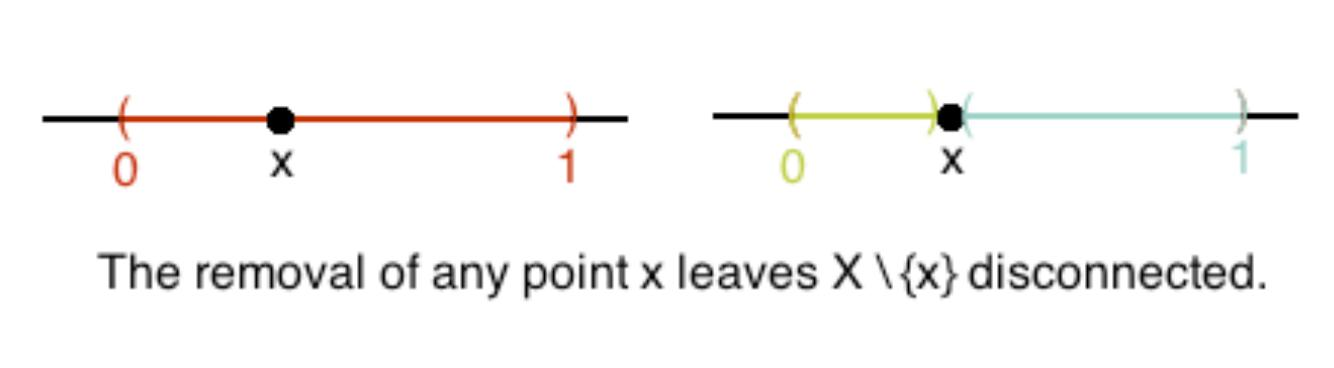
\includegraphics[scale = 0.3]{fotos_topo_1/exempleconnex1.jpeg}
\end{equation}
Però si traiem qualsevol punt $y\in Y$, $Y\setminus\{y\}$ segueix sent connex:
\begin{equation}
    \notag
    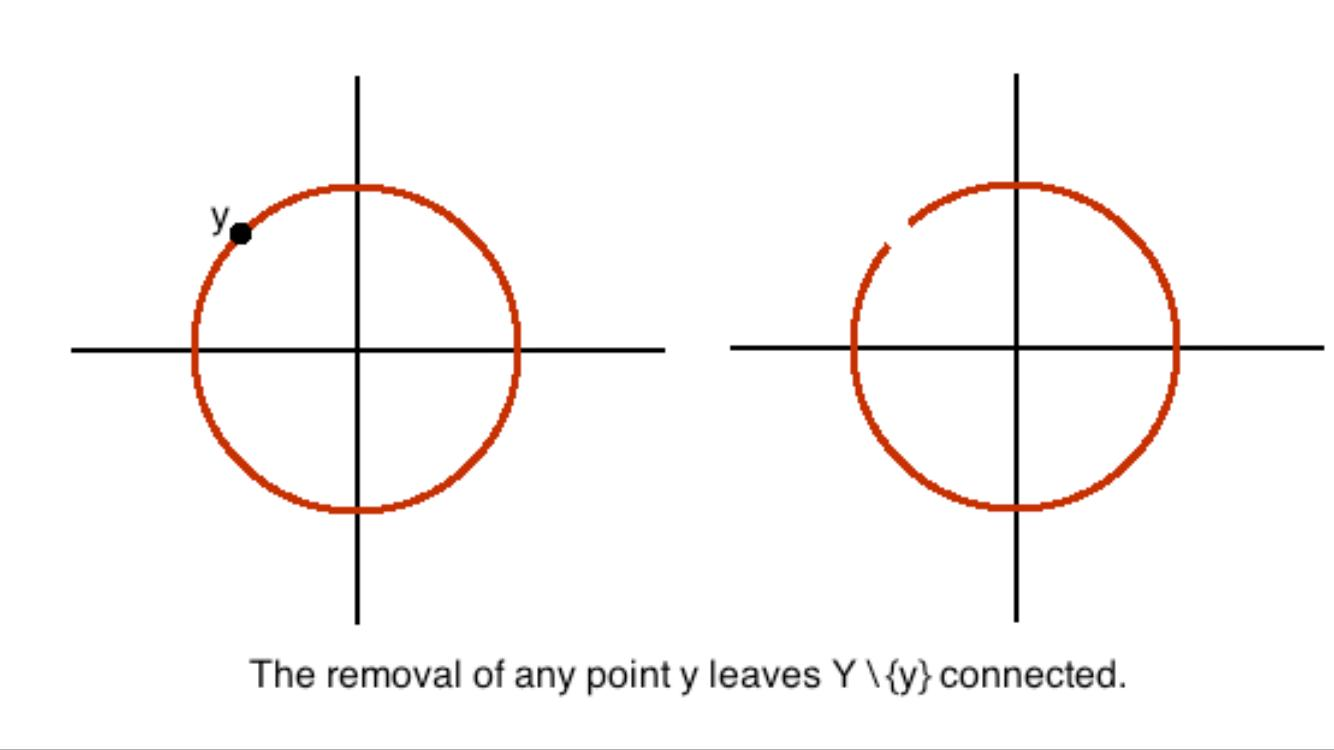
\includegraphics[scale = 0.3]{fotos_topo_1/exempleconnex2.jpeg}
\end{equation}
Llavors, per la proposició (\ref{prop:connexhomeomorf1}), $X\not\cong Y$.
\end{ej}





\subsection{Producte d'espais connexos}

Recordem que si $X,Y$ són espais topològics, definim una topologia sobre el producte cartesià $X\times Y$ a partir de la base $\beta = \{U\times V\;:\;U$ obert de $X,\;V$ obert de $Y\}$. Veurem que si $X$ i $Y$ són espais connexos, l'espai producte $X\times Y$ també ho és.

\begin{prop}
\label{prop:espaiproducteconnex1} Siguin $X$ i $Y$ espais topològics tals que $X$ és connex. Sigui $b\in Y$ i dotem al singletó $\{b\}$ de la topologia subespai de $Y$. Aleshores el producte $X\times \{b\}$ és connex.
\end{prop}
\begin{proof}
Suposem que és fals. Suposem que $X\times \{b\}$ és inconnex. Aleshores existeixen oberts $U_1\times V_1$, $U_2\times V_2$ de $X\times \{b\}$ tals que $(U_i\times V_i)\not=\emptyset$ i $(U_1\times V_1)\cup (U_2\times V_2) = X\times \{b\}$. Notem que $V_1,V_2\not=\emptyset$ ja que $U_i\times V_i\not=\emptyset$. Bé, doncs l'únic obert de $\{b\}$ (amb la topologia subespai) és $\{b\}$, per tant $V_1=V_2=\{b\}$ i per tant $\forall i=1,2$, $U_i\times V_i = U_i\times \{b\}$, i com $(U_1\times\{b\})\cap (U_2\times\{b\}) = \emptyset$ hem de tenir que $U_1,Y_2\subset X$, $U_1,U_2\not=\emptyset$ i $U_1\cap U_2 = \emptyset$. Notem que
\begin{equation}
    \notag
    X\times \{b\} = (U_1\times\{b\})\cup(U_2\times \{b\}) = (U_1\cup U_2)\times\{b\} .
\end{equation}
Això implica que $X = U_1\cup U_2$ i per tant $\{U_1,U_2\}$ és una separació de $X$ cosa que implica que $X$ és inconnex i això és una contradicció. Així doncs, hem provat cert el resultat.
\end{proof}

\begin{prop}
\label{prop:espaiproducteconnex2} Sigui $\{X_1,\ldots,X_n\}$ una col·lecció finita d'espais topològics connexos. Aleshores, el producte $X_1\times\cdots\times X_n$ és connex.
\end{prop}
\begin{proof}
Provarem el cas per $n = 2$ i diré $X = X_1$ i $Y = X_2$ per anar més ràpid. Considerem, doncs, $X$ i $Y$ dos espais topològics connexos qualssevol i sigui $(a,b)\in X\times Y$. Com $X$ és connex, $X\times \{b\}$ també és connex per la proposició anterior. De manera similar, per tot $x\in X$, $\{x\}\times Y$ és connex. Definim
\begin{equation}
    \notag
    T_x = (X\times\{b\})\cup(\{x\}\times Y)
\end{equation}
\begin{equation}
    \notag
    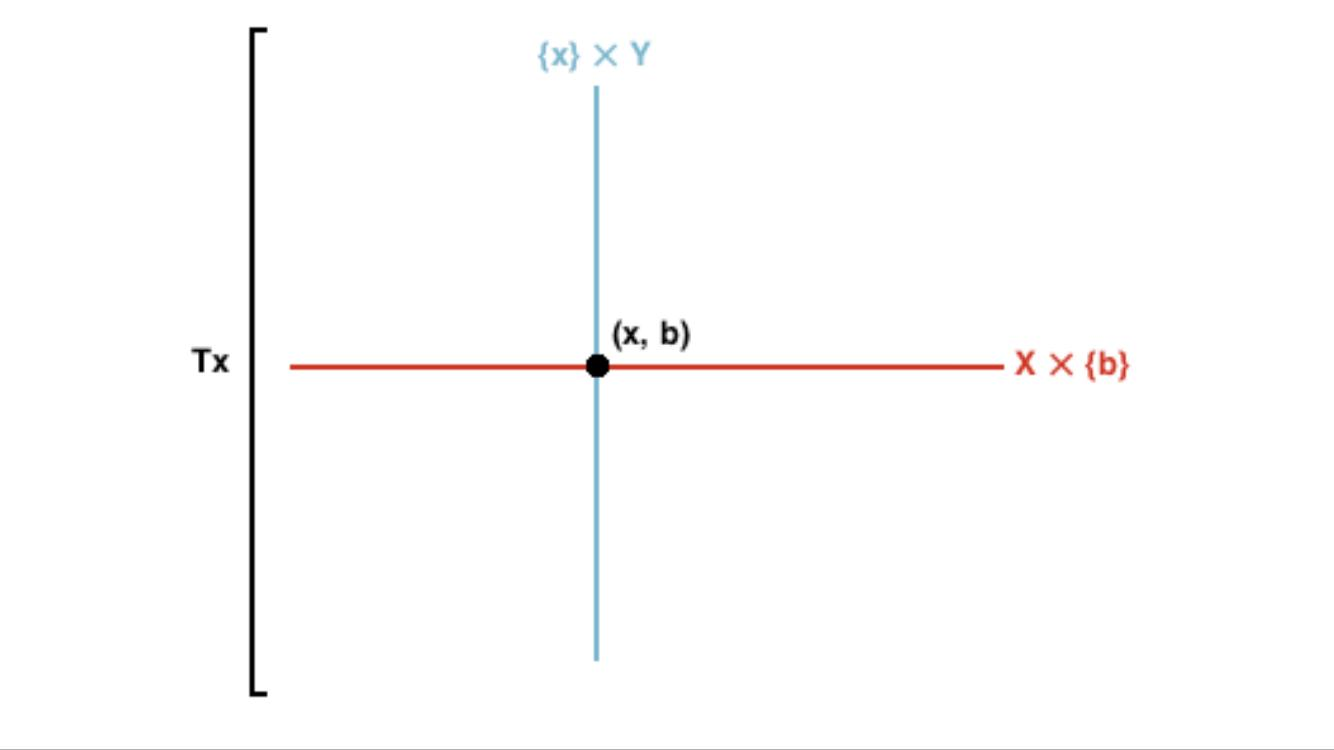
\includegraphics[scale = 0.3]{fotos_topo_1/producteconnexos.jpeg}
\end{equation}
Notem que $T_x$ és connex pel terme del punt comú. Això és perquè cada $x\in X$, $(x,b)\in X\times \{b\}$ i $(x,b)\in \{x\}\times Y$. Aleshores
\begin{equation}
    \notag
    X\times Y = \bigcup_{x\in X} T_x = \bigcup_{x\in X}(X\times\{b\})\bigcup(\{x\}\times Y)
\end{equation}
Cada $T_x$ conté el punt $(a,b)$ ja que $(a,b)\in (X\times\{b\})\subset(X\times\{b\})\cup (\{x\}\times Y) = T_x$ i per la proposició mencionada, $X\times Y$ és connex.
\end{proof}



\subsection{Relació entre connexió i arc-connexió}

\begin{ter}
\label{ter:arcconneximplicaconnex} Si $X$ és arc-connex, aleshores $X$ és connex.
\end{ter}
\begin{proof}
Sigui $X$ un espai topològic connex i suposem que $X$ no és connex. Aleshores existeixen oberts $A,B\subset X$, on $A,B\not=\emptyset$, $A\cap B = \emptyset$ i $X = A\cup B$. Siguin $a\in A$ i $b\in B$. Com $X$ és arc-connex, existeix un camí amb punt inicial $a$ i punt final $b$, és a dir, existeix una aplicació contínua $\alpha:[0,1]\rightarrow X$ tal que $\alpha(0) = a$ i $\alpha(1) = b$. Com $\alpha$ és contínua, $\alpha^{-1}(A)$ i $\alpha^{-1}(B)$ són els dos oberts en $I = [0,1]$, satisfent $\alpha^{-1}(A),\alpha^{-1}(B) \not=\emptyset$ i com $A\cap B = \emptyset$, $\alpha^{-1}(A)\cap \alpha^{-1}(B)=\emptyset$. Finalment, com $X = A\cup B$,
\begin{equation}
    \notag
    [0,1] = \alpha^{-1}(X) = \alpha^{-1}(A\cup B) = \alpha^{-1}(A)\cup\alpha^{-1}(B)
\end{equation}
i això demostra que $\{\alpha^{-1}(A),\alpha^{-1}(B)\}$ és una separació de $I$, però $I$ és un subespai connex (amb la topologia subespai en $\mathbb{R}$) i per tant és una contradicció. $X$ ha de ser connex.
\end{proof}

\begin{nota}
\label{nota:connexnoimplicaarcconnex} Hem vist que arc-connex implica connex. Ara, però, la implicació contrària no és sempre certa. Considerem, per exemple, $X = \{(0,y)\in\mathbb{R}^2\;:\;-1\leq y\leq 1\}\cup\{(x,\sin(\pi/x))\;:\;x\in (0,1]\}$. 
\begin{equation}
    \notag
    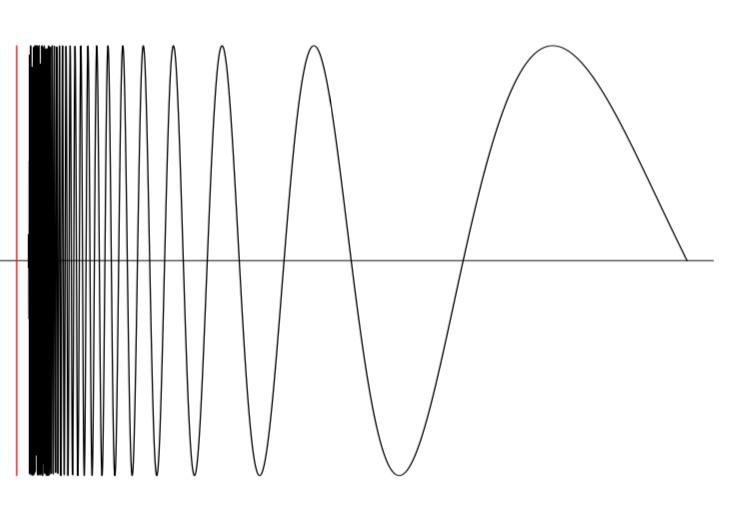
\includegraphics[scale = 0.3]{fotos_topo_1/localmentarcconnex.jpeg}
\end{equation}
Aquest espai topològic no és arc-connex ja que no existeix cap camí amb origen a $(1,0)$ i final en $(0,0)$. En canvi és connex. En efecte, $X$ és l'adherència de la imatge de la funció contínua $f:[0,1)\rightarrow \mathbb{R}^2,$ $f(x) = (x,\sin (\pi/x))$ que és connexa. La connexió de $X$ és conseqüència del lema (\ref{lema:recobrimentsconnex}).
\end{nota}

Veiem un cas particular on connex implica arc-connex.

\begin{prop}
\label{prop:conneximplicaarcconnex} Si $A$ és un obert connex de $\mathbb{R}^n$ (amb la topologia euclidiana) aleshores $A$ és arc-connex.
\end{prop}
\begin{proof}
Sigui $\mathbb{R}^n$ amb la topologia usual euclidiana i sigui $A\subseteq \mathbb{R}^n$ un subespai connex. Siguin $x,y\in A$ i sigui $\mathcal{R}$ la família de boles obertes contingudes en $A$.
\begin{equation}
    \notag
    \mathcal{R} = \{B = B(x,r)\;:\;x\in A,\;r>0,\;B(x,r)\subset A\}
\end{equation}
Com $A$ és obert i $x\in A$ existeix una bola oberta continguda en $\mathcal{R}$ que conté $x$, sigui $B_1 = (x,r_x)$.
\begin{equation}
    \notag
    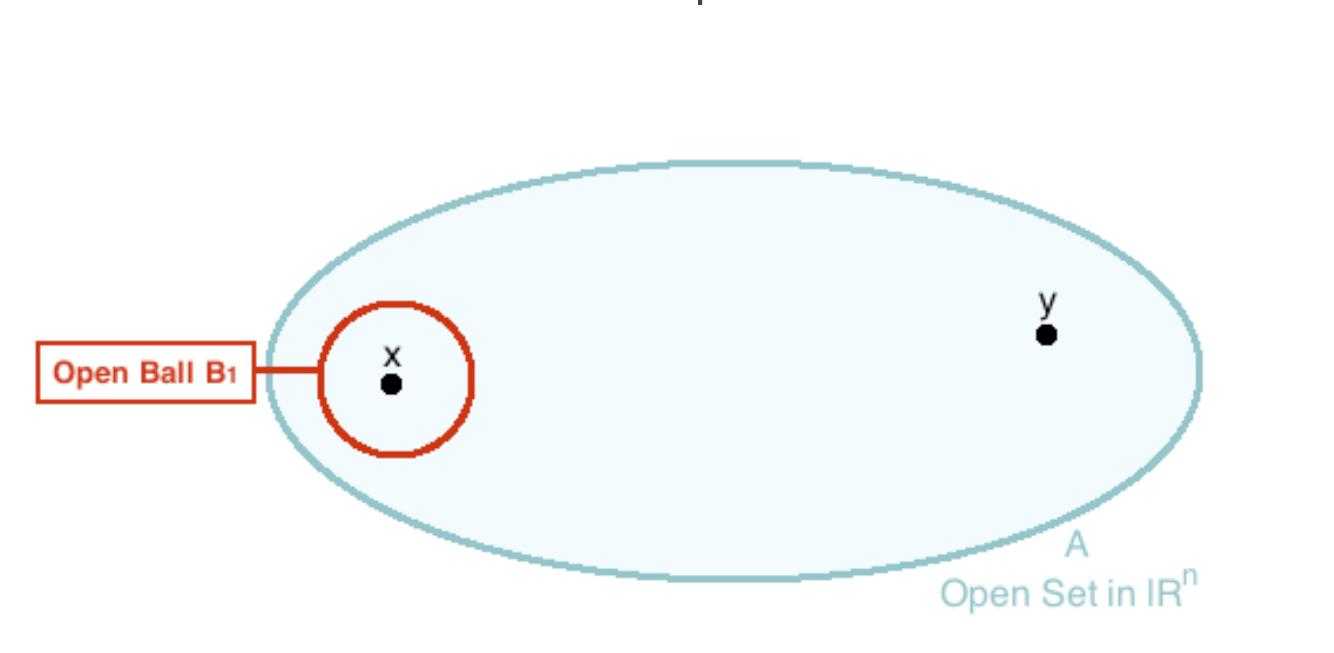
\includegraphics[scale = 0.2]{fotos_topo_1/conneximplicaarcconnex1.jpeg}
\end{equation}
Sigui $B_2$ la unió de totes les boles obertes de $\mathcal{R}$ tals que $B\cap B_1\not=\emptyset$,
\begin{equation}
    \notag
    B_2 = \{\bigcup_{B\in\mathcal{R}}B \;:\;B\cap B_1\}
\end{equation}
\begin{equation}
    \notag
    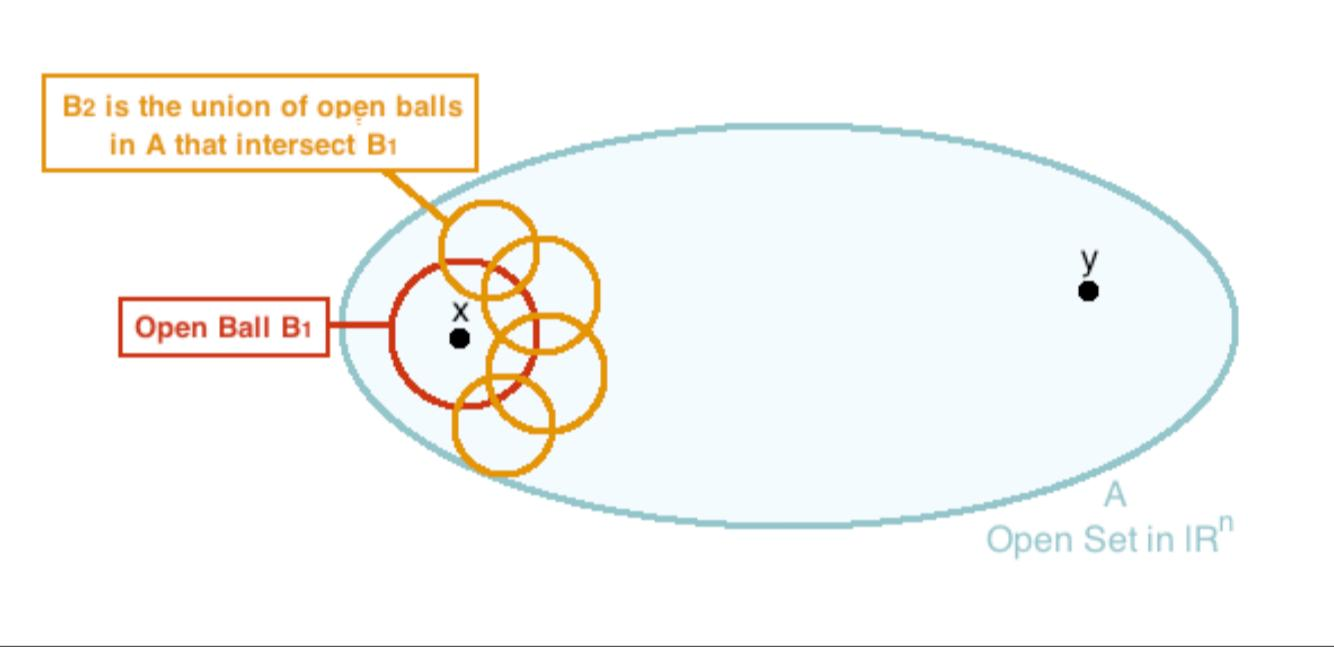
\includegraphics[scale = 0.2]{fotos_topo_1/conneximplicaarcconnex2.jpeg}
\end{equation}
En general, $\forall i\in \mathbb{N}$, $i>1$, sigui $B_i$ la unió de totes les boles tals que 
\begin{equation}
    \notag
    B_i = \{\bigcup_{B\in\mathcal{R}}B\::\;B\cap B_{i-1}\not=\emptyset\}
\end{equation}
\begin{equation}
    \notag
    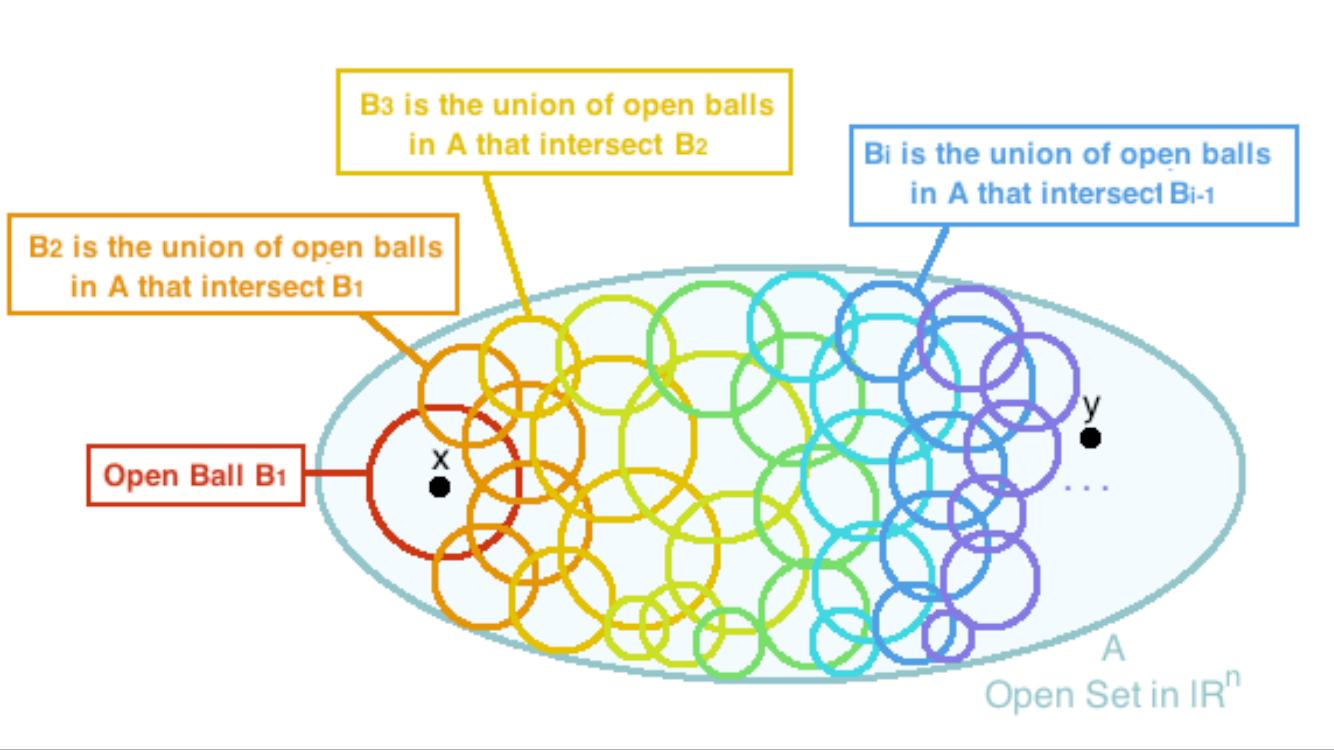
\includegraphics[scale = 0.2]{fotos_topo_1/conneximplicaarcconnex3.jpeg}
\end{equation}
Ara afirmem que cada bola $B\in\mathcal{R}$ està continguda en alguna $B_i$. Suposem que no, sigui $V = \bigcup_{i=1}^\infty B_i$ i sigui $W = \bigcup_{B\in\mathcal{R}^*}B$ on 
\begin{equation}
    \notag
    \mathcal{R}^* = \{B\in\mathcal{R}\;:\;B\not\subseteq B_i,\;\forall i\in I\}
\end{equation}
Aleshores $V$ i $W$ són els dos oberts ja que són la unió de boles obertes. A més $V,W\not=\emptyset$, $V\cap W=\emptyset$ i $A = V\cup W$. Per tant, $\{W,V\}$ és una separació d'$A$ però això és una contradicció. Per tant, $\forall B\in\mathcal{R}$, $\exists i\in\{1,2,\ldots\}$ tal que $B\subseteq B_i$. Llavors, $\exists n\in\{1,2,\ldots\}$ tal que $y\in B_n$. A més, $A = V = \bigcup_{i=1}^\infty B_i$ és tal que $B_i\cap B_{i+1}\not=\emptyset$, $\forall i$. Aleshores, per la proposició (\ref{prop:arcconnex3}) $V=A$ és arc-connex.
\end{proof}

\begin{prop}
\label{prop:conneximplicaarcconnex2} Sigui $X$ un espai topològic connex i localment arc-connex. Aleshores és arc-connex.
\end{prop}
\begin{proof}
Fixem un punt $x\in X$. N'hi haurà prou en veure que tot punt $y\in X$ es pot arc-connectar amb $x$. És a dir, que 
\begin{equation}
    \notag
    A = \{y\in X\;:\;\text{$y$ es pot arc-connectar amb $x$}\}
\end{equation}
és igual a $X$. Notem que $x\in A$ i, per tant, $A\not=\emptyset$ Sigui $y\in A$, i sigui $V$ un entorn arc-connex del punt $y$. Tots els punts de $V$ es poden arc-connectar amb $y$ que, al mateix temps es pot arc-connectar amb $x$. Com que l'arc-connexió és una relació d'equivalència, obtenim que $V\subset A$ i, en conseqüència, que $y$ és interior a $A$. Això prova que $A$ és obert. Veiem que $A$ és també tancat: si $z\in (X\setminus A)$ i $W$ és un entorn arc-connex de $z$, aleshores $W\cap A=\emptyset$. En cas contrari, existirien punts arc-connectats amb $x$ i amb $z$, la qual cosa contradiu que $z\not\in A$. Així, $W\subset X\setminus A$ i $z$ és interior a $X\setminus A$. Això implica que $(X\setminus A)^{o} = X\setminus A$ i per tant és obert. És a dir, $A$ és tancat. Com que $A$ és obert i tancat i $A\not=\emptyset$ en un espai connex, per la proposició (\ref{prop:criterideconnexio1}) deduïm que $A = X$.
\end{proof}

\subsection{Components connexes}

\begin{defi}[Connectats]
\label{def:connectats}\index{Connectats} Sigui $X$ un espai topològic. Diem que dos punts de $X$ estan \textit{connectats} si existeix un subconjunt connex de $X$ que conté els dos punts.
\end{defi}

\begin{prop}
\label{prop:relacioconnexio} Sigui $X$ un espai topològic. La relació $x$ ``està connectat amb'' $y$ és d'equivalència.
\end{prop}
\begin{proof}
Clarament $x$ està connectat amb sí mateix i si $x$ està connectat amb $y$, òbviament $y$ està connectat amb $x$. Si $x$ està connectat amb $y$ i $y$ amb $z$, aleshores existeixen connexos tals que $x,y\in A$ i $y,z\in B$. Aleshores $A\cup B$ és connex ja que $y\in A\cap B\Rightarrow A\cap B\not=\emptyset$. Per tant $A\cup B$ és un connex contenint $x$ i $z$.
\end{proof}

\begin{defi}
[Component connexa]\label{def:componentconnexa}\index{Component connexa} Sigui $X$ un espai topològic i sigui $x$ un punt de $X$. La \textit{component connexa} de $x$ és \begin{equation}
    \notag
    c(x) := \{y\in X\;:\;\text{$y$ està connectat amb $x$}\}
\end{equation}
\end{defi}

Observem que $X$ és reunió disjunta de components connexos.

\begin{prop}
\label{prop:componentconnexa1} Sigui $X$ un espai topològic. La component connexa d'un punt $x\in X$ és el subespai connex de $X$ més gran que conté $x$. En particular, $ca(x)\subset c(x)$ i $c(x)$ és un tancat.
\end{prop}
\begin{proof}
Per a tot $y\in c(x)$, existeix un connex $A_y$ que conté $x$ i $y$. Aleshores, $c(x) = \bigcup_{y\in c(x)}A_y$ és connex. Si $K\subset X$ és connex i $x\in K$, aleshores tots els punts de $K$ estan connectats amb $x$ i, per tant $K\subset c(x)$. Com que $ca(x)$ és arc-connex, per (\ref{ter:arcconneximplicaconnex}) és connex, i com que conté $x$ tenim que $ca(x)\subset c(x)$. D'altra banda, $\overline{c(x)}$ és també un connex que conté $x$. Així $c(x) = \overline{c(x)}$ (ja que per definició de clausura tenim $c(x)\subset\overline{c(x)}$ i com que $c(x)$ és el connex més petit que conté a $x$, se satisfà la inclusió contrària).
\end{proof}

En general les components connexes no són obertes. Per exemple
\begin{equation}
    \notag
    c(x) = \{x\in\mathbb{R}\;:\;x = 0\;\text{ó}\;x=1/n,\;n\geq 0\}
\end{equation}

\begin{prop}
\label{prop:componentconnexa2} Les components connexes d'un espai topològic localment arc-connex són oberts.
\end{prop}
\begin{proof}
Sigui $x\in X$ i sigui $y\in c(x)$. Sigui $V$ un entorn arc-connex (i, per tant, connex) del punt $y$. Aleshores $c(x)\cup V$ és reunió de dos conjunts connexos no disjunts (ja que $y\in c(x)\cap V$). Per la maximalitat de $c(x)$, tenim que $c(x)\cup V\subset c(x)$. Així $y\in V\subset c(x)$. Per tant $y$ és interior a $c(x)$.
\end{proof}



























%%%%%%%%%%%%%%%%%%%%%%%%%%%%%%%%%%%%%%%%%%%%%%%%%%%%%%%%%%%%%%%%%%%%%%%%%%%%%%%%%%%%%%%%%%%%%%%%%%%%%%%%%%%%%%%%%%%%%%%%%%%%%%%%%%%%%%%%%%%%









%%%%%%%%%%%%%%%%%%%%%%%%%%%%%%%%%%%%%%%%%%%%%%%%%%%%%%%%%%%%%%%%%%%%%%%%%%%%%%%%%%%%%%%%%%%%%%%%%%%%%%%%%%%%%%%%%%%%%%%%%%%%%%%%%%%%%%%%%%%%

































































\end{document}